\chapter{Case Study}
When talking about animal movement behavioural animals might use a reaction-diffusion process. This process entails the movement (diffusion) and the interaction with the environment (reaction). Reaction is often described as finding food, mating a mate or finding a predator. All of these things force the animal into changing its movement behaviour. This could mean a stop in a long search for example. Reaction behaviour will not be a part of this report.

\section{Diffusion processes}
Diffusion processes can also be called walks. This section seeks to explain some of the different walks and what is characteristic about them.

\subsection{Brownian motion}
Brownian motion is a type of random walk where the motion follows a Gaussian distribution. In mathematically terms this can be shown as follows:
\begin{equation}
P($Step size$) \sim \mathcal{N}(0,t-s) ($for $ 0 \leq s \leq t)
\label{eq:brownianm}
\end{equation}
This type of diffusion where the variance grows over time is called normal diffusion. Characteristic for the Brownian motion is that the walker will return to the same spot multiple times. This can be seen in a one dimensional model in figure \ref{fig:brownianrw}.
\begin{figure}[H]
\centering
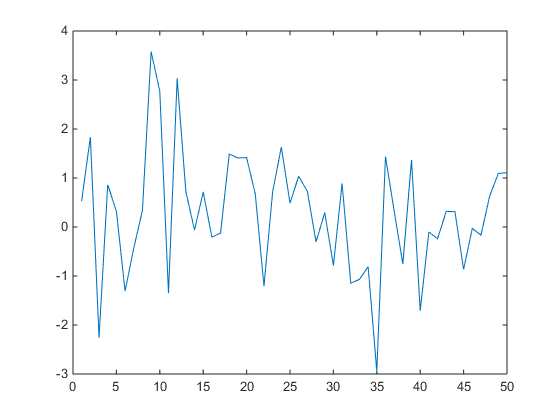
\includegraphics[width = 0.6\textwidth]{billeder/brownian}
\caption{Brownian Random Walk}
\label{fig:brownianrw}
\end{figure}
When looking at Brownian random walks it becomes apparent that the model might not reflect animal behaviour as it would be a bad strategy to visit the same area multiple times in a search. Only when you revisit a site with fast food regeneration would this strategy seem feasible.\\
Brownian motion obeys the rule of the central limit theorem. When the variance in equation \ref{eq:brownianm} gets sufficiently large the distribution will be very wide and the probability for $P(0)$ will be very low.

\subsection{Levy motion}
Lévy motion, also know as lévy flight or lévy walks, is a type of random walk where the step length generally follows a power law tailed distribution. In mathematically terms this can be shown as follows:
\begin{equation}
P($Step size$) \sim l ^{-\mu} ($for $ 0 < l $, $1 < \mu < 3$ and $ \mu = 1 + \alpha)
\label{eq:levyrw}
\end{equation}
In equation \ref{eq:levyrw} the $\alpha$ is the characteristic exponent. When the number of steps gets sufficiently large the distances converges to a stable distribution. Both distributions are fat tailed allowing large step sizes which would otherwise be classified as outliers in a Gaussian distribution. A two dimensional model of a levy flight can be seen in figure \ref{fig:levywalk1}.
\begin{figure}[H]
\centering
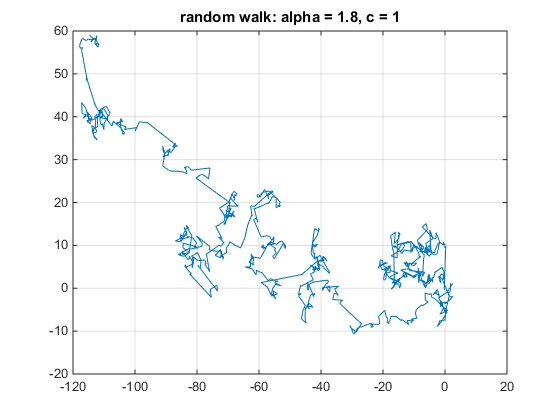
\includegraphics[width = 0.6\textwidth]{billeder/levywalk1}
\caption{Levy flight with 1000 steps and $\alpha = 1.8$}
\label{fig:levywalk1}
\end{figure}

\section{The Lévy alpha-stable distribution}
The skew Lévy $\alpha$-stable distribution is the most general case of stable distributions. The characteristic function is given by:
\begin{equation}
\varphi (t) = exp[itv - |ct|^{\alpha} (1-i\beta sign(t) tan[\frac{\alpha \pi}{2}])] $, for $ \alpha \neq 1
\end{equation}
and
\begin{equation}
\varphi (t) = exp[itv - |ct|^{\alpha} (1-i\beta sign(t) -(\frac{2}{\pi})ln|t|)] $, for $ \alpha = 1.
\end{equation}
where $i$ is the imaginary i, $v$ is the location parameter, $c$ is the scaling parameter, $\alpha$ is the characteristic exponent (or stability parameter) and $\beta$ is the skewness parameter. The ranges of these parameters are:\\
\begin{center}
$\alpha \in (0, 2]$\\
$\beta \in [-1, 1]$\\
$c \in (0, \infty)$\\
$v \in (-\infty, \infty)$\\
\end{center}
The characteristics for stable distribution entail when $\alpha = 2$ the distribution is reduced to a Gaussian distribution with variance $\sigma^2 = 2c^2$ and when $\alpha = 1$ and $\beta = 0$ the distribution is reduced to a Cauchy distribution. The variance is only defined when $\alpha = 2$. The mean is only defined when $1 < \alpha $ then the mean is equal to $v$.\\
The Probability Density function is found by Fourier transforming the characteristic function.\\
\begin{equation}
P(S) = \frac{1}{2\pi}\int_{-\infty}^{\infty} \varphi(t) exp[-itS] dt
\end{equation}
The most simple version of the characteristic function is when $\beta = 0$ and $v = 1$. The characteristic function is reduced to:
\begin{equation}
\varphi (t) = exp[- |ct|^{\alpha}]
\label{eq:reducedcharfunc}
\end{equation}
It is then said that the distribution is a symmetric alpha-stable distribution or S$\alpha$S. The symmetry can be seen in figure \ref{fig:stablepdfsweep} where $\alpha$ is swept from 0.2 to 2. 
\begin{figure}[H]
\centering
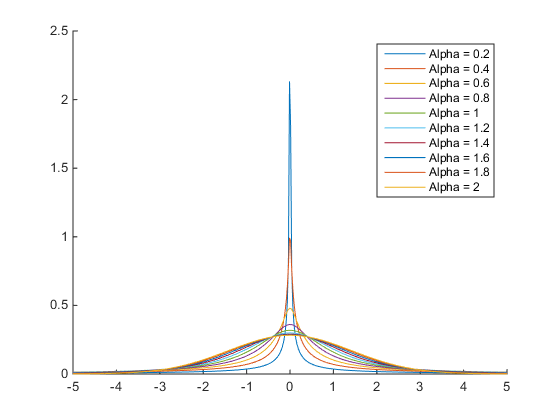
\includegraphics[width = 0.8\textwidth]{billeder/stblpdfsweep}
\caption{Stable distribution sweep of $\alpha$}
\label{fig:stablepdfsweep}
\end{figure}
The function seen in equation \ref{eq:reducedcharfunc} will be the basis of the simulation done in this study.

\section{Matlab simulation}
 
